\documentclass[11pt]{article}
\usepackage{mathtools,hyperref,booktabs,fullpage}
%\usepackage[amssymb,cdot]{SIunits}
%\usepackage[utopia]{mathdesign}     
\usepackage{xcolor}
\usepackage{amsmath}
\usepackage{amssymb}
\usepackage{hyperref}
\usepackage{longtable}
\usepackage{fullpage}
\usepackage{listings}
\usepackage{enumitem}
\setlist{nolistsep}


\usepackage{listings}
\usepackage{color}
\definecolor{dkgreen}{rgb}{0,0.6,0}
\definecolor{gray}{rgb}{0.5,0.5,0.5}
\definecolor{mauve}{rgb}{0.58,0,0.82}
\definecolor{lightgray}{rgb}{0.9,0.9,0.9}
\lstset{language=Python,
  aboveskip=3mm,
  belowskip=3mm,
  showstringspaces=false,
  columns=flexible,
  basicstyle={\ttfamily},
  numbers=left,
  numberstyle=\small\color{gray},
  keywordstyle=\color{blue},
  commentstyle=\color{dkgreen},
  stringstyle=\color{mauve},
  breaklines=true,
  breakatwhitespace=true,
  tabsize=3
}


%\definecolor{lightgray}{gray}{0.93}

\pagestyle{empty}
\setlength\parindent{0pt}
\renewcommand{\thefootnote}{\fnsymbol{footnote}}
 
\makeatletter
\renewcommand\section{\@startsection{section}{1}{\z@}%
                                  {-3.5ex \@plus -1ex \@minus -.2ex}%
                                  {2.3ex \@plus.2ex}%
                                  {\normalfont\bfseries}}
\makeatother


\begin{document}

{\large
  \begin{center}
    {\bf ME 701 -- Development of Computer Applications In Mechanical Engineering \\ 
         Homework 6  -- Due 10/25/2017 \\
    }
  \end{center}

\setlength{\unitlength}{1in}

}

\vspace{12pt}

\fbox{
  \parbox{0.95\textwidth}{
\textcolor{purple}{{\bf Instructions}}: 
  One TAR file  {\tt lastname\_firstname.tar} that contains two
  Python files:  {\tt lastname\_firstname\_hw6\_p1.py} 
  and {\tt lastname\_firstname\_hw6\_p2.py}, one for each 
  of the problems below.
  }
}



% Chapters 1,2,3



\section*{Problem 1}

Consider the following contour plot (from D.S.~McGregor et al.~NIM A {\bf 343} (1994)):

\begin{figure}[ht]
    \centering
    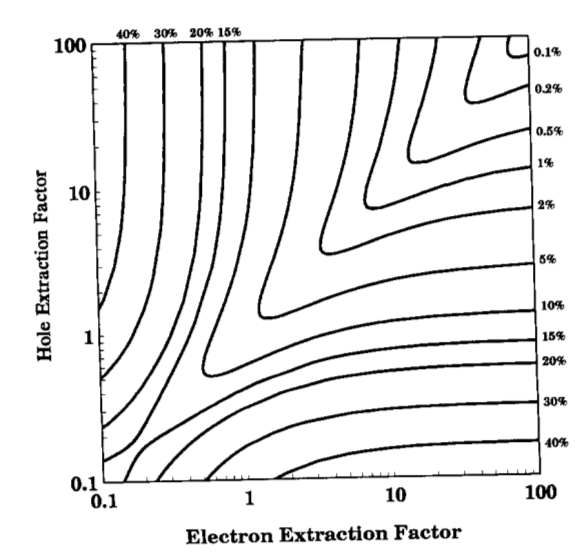
\includegraphics[keepaspectratio, width = 3.0 in]
                    {original_contour}
\end{figure}

In class, I proposed the following solution (also available in the 
examples repository):

\lstinputlisting[language=Python]{advanced.py}

Execution of the code leads to the following:

\begin{figure}[ht]
    \centering
    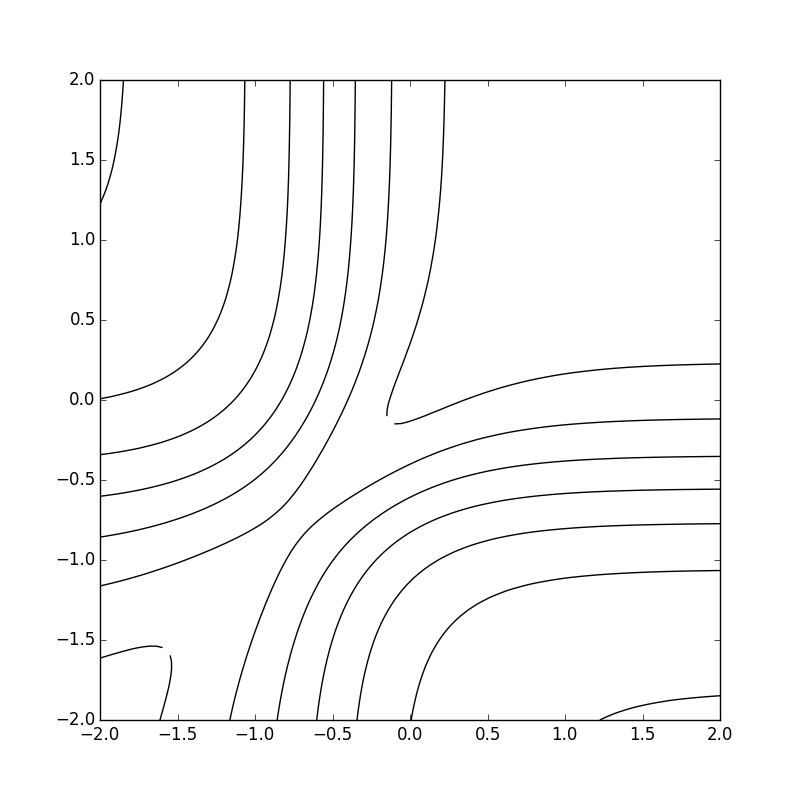
\includegraphics[keepaspectratio, width = 3.0 in]
                    {new_contour}
\end{figure}

This is on the right track, but several features are missing.  Your job
is to add the following:
\begin{enumerate}
 \item {\bf appropriate axis labels} (e.g., `Electron Extraction Factor')
 \item correct contour levels (i.e., 0.1, 0.2, 0.5, 1\%, and so on).
       {\it Hint}: look up the documentation for {\tt plt.contour}.
 \item {\bf correct $x$  and $y$ tick values} (e.g., -1 should be 0.1 and 2
       should be 100) {\it Hint}: look up, e.g., {\tt plt.xticks}.
 \item {\bf annotations for each contour line}. {\it Hint}: look up 
       {\tt plt.text}, paying specific attention to {\tt fontsize},
       {\tt horizontalalignment}, and {\tt verticalalignment}. 
       You might also which to consider using {\tt scipy.optimize.newton}
       to help you automatically find where text should be located,
       e.g., you know that the upper-left 40\% box should be located where 
       $F(x) = 100 - R(\rho_e, 100) = 0$.  However, you may simply
       place each text annotation manually.  (+1/2 point if you use newton or equivalent)
 \item {\bf logarithmic minor tick marks}.   Note the 
       original has minor tick marks spaced logarithmically, whereas
       my solution has no minor tick marks.  {\it Hint}: look 
       up {\tt plt.gca().yaxis}.
\end{enumerate}



\section*{Problem 2}

We are interested in examining how a time dependent problem changes with a parameter.  We shall investigate the time dependent heat transfer equation in 1-D, i.e.,
\begin{equation}
    \frac{\partial T}{\partial t} = \alpha \frac{\partial^2 T}{\partial x^2}\, ,
\end{equation}
with the boundary conditions that the $T(x=0)=1$ for all time $t$ and that $T(x=1) = 0$ for all time $t$.  We know that after an infinite amount of time, the solution is linear in $x$, but how do the solutions vary for a fixed time.  Here's a short program for doing that:

\lstinputlisting[language=Python]{heat.py}



Your task is to produce an animation showing how the solution changes with increasing alpha.  Explore the parameter range $\alpha\in[0,1]$. \\
 


\end{document}
